\capitulo{5}{Aspectos relevantes del desarrollo del proyecto}
%%%%%%%%%%%%%%%%%%%%%%%%%%%%%%%%%%%%%%%%%% Borrar
\begin{comment}
Este apartado pretende recoger los aspectos más interesantes del desarrollo del proyecto, comentados por los autores del mismo.
Debe incluir desde la exposición del ciclo de vida utilizado, hasta los detalles de mayor relevancia de las fases de análisis, diseño e implementación.
Se busca que no sea una mera operación de copiar y pegar diagramas y extractos del código fuente, sino que realmente se justifiquen los caminos de solución que se han tomado, especialmente aquellos que no sean triviales.
Puede ser el lugar más adecuado para documentar los aspectos más interesantes del diseño y de la implementación, con un mayor hincapié en aspectos tales como el tipo de arquitectura elegido, los índices de las tablas de la base de datos, normalización y desnormalización, distribución en ficheros3, reglas de negocio dentro de las bases de datos (EDVHV GH GDWRV DFWLYDV), aspectos de desarrollo relacionados con el WWW...
Este apartado, debe convertirse en el resumen de la experiencia práctica del proyecto, y por sí mismo justifica que la memoria se convierta en un documento útil, fuente de referencia para los autores, los tutores y futuros alumnos.

\end{comment}
%%%%%%%%%%%%%%%%%%%%%%%%%%%%%%%%%%%%%%%%%% COMIENZO

En este punto se recogerán los aspectos más relevantes del desarrollo comentando en cada caso las decisiones tomadas para llegar a nuestros objetivos haciendo un resumen de la experiencia práctica del proyecto, de cómo se solucionaron los problemas encontrados en cada caso y la relevancia que tuvieron en el alcance total del proyecto.

\section{Motivación del proyecto}
El proyecto se me ocurrió hace años cuando me emancipé a una vivienda con las persianas motorizadas que me parecieron que podrían hacer una función mayor si dispusieran de cierto equipamiento, y cogió fuerza con la llegada de la pandemia de la COVID19 cuando el tema surgió en distintas conversaciones en las que que había quien no podía acercarse a sus segundas viviendas y estaban preocupados por una posible ocupación. Tras darle vueltas a esta situación surgió la idea de crear un sistema domótico para poder ayudar a quien lo precise con este proyecto.

\section{Formación necesaria}
El proyecto requirió muchas horas de búsqueda de ideas por la web, ya que no existe información fiable de cómo realizar una instalación de estas características sino que existen muchos pequeños proyectos amateur que se centran en cubrir una pequeña necesidad; siendo proyectos que no disponen de un respaldo documental detrás. Abundan las soluciones de profesionales de otros campos que quieren probar a hacer sus propias soluciones de carácter amateur.

Por ello, para poder desarrollar el proyecto me vi en la necesidad de visitar numerosas páginas web de distinta índole para hacerme a la idea de cómo podría enfocar el proyecto. Aunque, el mayor hándicap a la hora de realizar este proyecto es la desinformación, por lo que me apoyé sobre todo en el REBT~\ref{concepto:RETB}~\cite{manual:REBT} y en mis conocimientos básicos de motores fruto de formación pasada.

La información de cómo funcionan los GPIO la obtuve tras realizar el curso de: “Control de GPIO con Python en Raspberry Pi” de Programo Ergo Sum~\cite{misc:programoergosum}.
Aunque, en parte la información de la web de \url{bujarra.com}~\cite{misc:BujarraGPIO} está desactualizada, esta publicación me ayudó a comprender cuál era el funcionamiento real de un relé y como conectarlo a los GPIO.

Otro punto importante a la hora de enfocar correctamente el proyecto fue el estudio del REBT~\cite{manual:REBT}, de su apartado BT-21~\cite{manual:ICT-BT-21}, del reglamento de ICT~\cite{manual:ICT} y los estándares de comunicaciones como son el IEEE802.11~\cite{manual:IEEE802.11} y el TIA568~\cite{manual:568.1}~\cite{manual:568.2}. Creo necesario confrontar estas normativas para poder realizar un proyecto a nivel profesional y documentalmente respaldado.

\section{Metodología}
Se eligió Scrum como la metodología global sobre la que realizar el proyecto de forma iterativa y ágil. Buscamos generar un proyecto lo más cercano a cómo sería un proyecto de este tipo en el ámbito laboral, pero salvando las distancias con un grupo de trabajo real con el que poder interactuar. Aunque he tenido reuniones semanales con los tutores no se ha realizado un seguimiento diario pero sí se cumplieron, en cualquier caso, unas reglas generales mínimas:

\begin{itemize}
    \item Los trabajos se desarrollaron en forma de <<sprints>> semanales.
    \item Tras cada <<sprint>> semanal se realiza una entrega de trabajo de forma incremental.
    \item En cada revisión del <<sprint>> se disponen los trabajos a realizar durante la semana.
    \item Realizando una revisión semanal, el proyecto goza de flexibilidad al integrar cambios sobre trabajos pequeños de forma que el proyecto está en constante mejora.
    \item Sobre el Kanban se realiza la estimación de tiempos por tareas según dificultad.
    \item Se priorizan las tareas del proyecto según mayor valor de negocio.
    \item Se cambia el estado de los <<issues>>, mediante un Kanban, según evoluciona el trabajo.
    \item Comprobamos como avanza el proyecto con los gráficos BurnDown de que dispone Zenhub.
\end{itemize}

Reseñar que en las fases de trabajos físicos no se ha aplicado Scrum pero se ha realizado con un criterio lo más cercano posible. Por ello, se predispuso realizar la tirada de cable y el conexionado la misma semana para que pudiera integrarse lo mejor posible en la metodología.

\section{Desarrollo del proyecto}
A medida que el proyecto ha ido tomando forma también se han ido implementando cambios: La idea original del proyecto era parametrizar los elementos según horas pero posteriormente se valoró e implantó la idea de tomar datos externos para poder controlar los elementos del sistema domótico. El proyecto se ha creado de forma cronológica siguiendo los pasos que se desarrollan a continuación.

El proyecto se comenzó por los scripts de extracción de datos para comprobar que se podía realizar el software que se había propuesto antes de continuar ya que es más fácil presentar cambios al principio que cuando el proyecto está avanzado. Aunque cabe destacar que se ha invertido una gran cantidad de tiempo en la búsqueda de información y normativas que desconocía, así como en la extracción y el tratamiento de datos.

Por tanto, se comenzó extrayendo datos desde Python~\cite{misc:Python} mediante web scraping~\ref{4:WebScraping} pero nos dimos cuenta de que una web es más susceptible de sufrir cambios. Por ello, recurrimos a APIS de terceros sin coste para poder realizar dicha extracción de datos, y tratándolos como json~\cite{misc:Json} extraer los datos que nos interesen.

\subsection{Extracción de datos}
Los algoritmos de extracción y tratamiento de datos también han ido cambiando ya que se han ido modificando las APIS para obtener más datos y de carácter más fiable.

Al comenzar a extraer datos de la API de geolocalización de~\url{www.ifconfig.me/ip} me obtenía la ubicación de la provincia, lo cual no es nada exacto ya que tendremos temperaturas diferentes según ubicación. Por ello, me vi obligado a hacer una búsqueda más a fondo para encontrar una API que se ajustase a las necesidades del proyecto. Tardé algunos días hasta que encontré \url{http://ip-api.com} que me entregaba más información y más fiable. Además, en el mismo intervalo, pasamos de utilizar web scraping a tratar los datos directamente como json~\cite{misc:Json}, que también es un cambio importante.

\begin{figure}
    \centering
    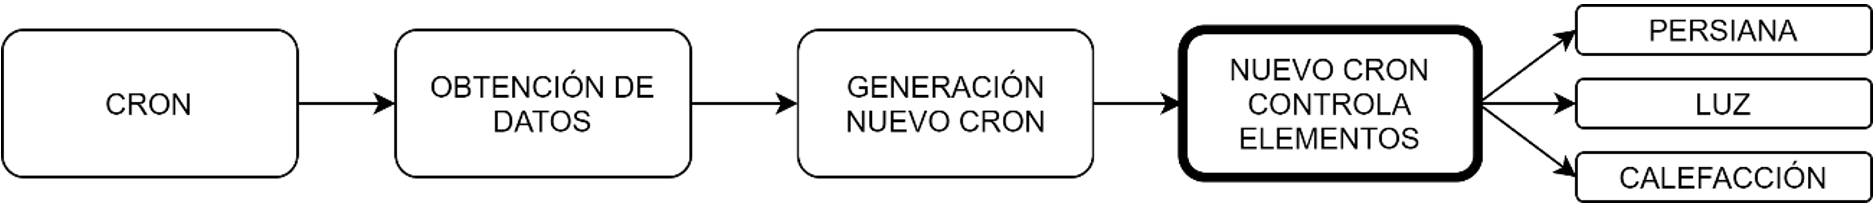
\includegraphics[width=\textwidth]{img/Cron1.PNG}
    \caption{Proceso de obtención de datos, programación de tareas y ejecución.} \label{Img:Cron1}
\end{figure}

En la segunda API, en el caso de~\url{www.weatherapi.com} podía obtener únicamente los valores de salida y puesta de sol para realizar el control de las persianas pero también era insuficiente, por lo que tuve que volver a hacer una búsqueda más amplia hasta que encontré~\url{www.climacell.co}, que me entrega las temperaturas de las próximas horas además de otros muchos parámetros que pueden llegar a servirnos como, por ejemplo, la velocidad del viento o si será un día nublado.

Tras obtener la ubicación de la instalación y extraer los parámetros necesarios de las APIS pasamos a conformar el archivo de datos para generar la configuración de Cron (Cron, es el programador de tareas de Linux~\cite{misc:Linux}). Esta fase dispone de varios pasos:

\begin{enumerate}
    \item Desde <<Cron>> se llama al script de toma de datos.
    \item Conformamos el nuevo archivo de <<Cron>>.
    \item El nuevo <<Cron>> lanza los scripts según las horas predispuestas.
\end{enumerate}

De esta manera el control de los dispositivos se hará automáticamente desde <<Cron>> con los datos actualizados diariamente. Podemos ver un diagrama explicativo de este proceso en la imagen~\ref{Img:Cron1}. Además, podemos ver a continuación un ejemplo de archivo de recopilación de datos:

\begin{lstlisting}[language=json, basicstyle=\small, caption={Ejemplo archivo de recopilado de datos.}]
{
"Planeta":
	{
	"Amanecer": "08:37:00",
	"Anochecer": "17:57:00"
	},

"temperaturas":
	{
	"0": 5.26,
	"1": 5.78,
	"2": 5.93,
	"3": 5.95,
	"4": 5.97,
	"5": 5.76,
	"6": 4.72,
	"7": 3.79,
	"8": 3.38,
	"9": 3.98,
	"10": 5.3,
	"11": 6.58,
	"12": 7.46,
	"13": 8.47,
	"14": 8.78,
	"15": 8.89,
	"16": 7.91,
	"17": 6.58,
	"18": 5.66,
	"19": 5.05,
	"20": 4.43,
	"21": 3.85,
	"22": 3.37,
	"23": 2.91
	}
}
\end{lstlisting}


Este archivo de datos es leído siempre que queremos modificar alguno de los parámetros de automatización desde el bot, como son la temperatura o la hora más temprana a la que pueden bajar las persianas, además de cuando se regenera el Cron.

\subsection{Scripts}
Utilizaremos dos tipos de scripts, Bash~\cite{misc:Linux} y Python~\cite{misc:Python}.

Una vez determinados los datos que vamos a necesitar en un notebook de Jupyter debemos realizar la extracción de estas líneas de código a un script Python.
En este punto tuve un problema bastante sencillo de resolver: el script necesita importar librerías para hacerlo correr y necesitaba instalarlas. En principio, esto no debería ser un problema ya que sabemos que se puede instalar con Pip. El problema surge al tener instalado Python v2 y Python v3, ya que si instalas las librerías utilizando Pip no funcionarán con Python3. Así que, hay que instalarlas con Pip3 para poder utilizarlas desde Python3:
\begin{lstlisting}[language=cpp,firstnumber=0]
pip install paquete
\end{lstlisting}
\begin{lstlisting}[language=cpp,firstnumber=1]
pip3 install paquete
\end{lstlisting}

Controlaremos la Raspberry Pi y sus periféricos mediante comandos Bash y realizaremos el cocinado de datos con Python. Se ha tomado esta determinación para conseguir la mayor velocidad de procesamiento posible así como para evitar posibles problemas. Por ello, la automatización que haremos desde CRON que lanzará otros scripts será mediante bash. Podemos ver el resultado final del Cron que genera la máquina diariamente:

\begin{lstlisting}[language=cpp, basicstyle=\tiny, caption={Crontab funcionando correctamente.}]
# Edit this file to introduce tasks to be run by cron.
# 
##   Entry              Description     Equivalent To
##   @yearly    Run once a year at midnight in the morning of January 1 0 0 1 1 *
##   @monthly   Run once a month at midnight in the morning of the first of the month 0 0 1 * *
##   @weekly    Run once a week at midnight in the morning of Sunday 0 0 * * 0
##   @daily     Run once a day at midnight 0 0 * * *
##   @hourly    Run once an hour at the beginning of the hour 0 * * * *
##   @reboot    Run at startup  @reboot
##   
# For more information see the manual pages of crontab(5) and cron(8)
# 
#minute (0-59),
#| hour (0-23),
#| | day of the month (1-31),
#| | | month of the year (1-12),
#| | | | day of the week (0-6 with 0=Sunday).
#| | | | |   commands

#--------------------------------------------------------------------------
#Este CRON ha sido generado en el instante Sun Dec 27 13:13:27 2020
#--------------------------------------------------------------------------
#Codigo de control Automático de Persianas 
#--------------------------------------------------------------------------
#Subimos las persianas Modo mañana de Lunes a Domingo
37 8 * * * sh /home/pi/source/TFG/scripts/control/GPIO_off.sh
38 8 * * * sh /home/pi/source/TFG/scripts/control/Subir.sh
44 8 * * * sh /home/pi/source/TFG/scripts/control/GPIO_off.sh

#Encendemos las luces
7 18 * * * sh /home/pi/source/TFG/scripts/LucesOn.sh

#Bajamos TODAS
12 18 * * * sh /home/pi/source/TFG/scripts/control/GPIO_off.sh
13 18 * * * sh /home/pi/source/TFG/scripts/control/Bajar.sh
19 18 * * * sh /home/pi/source/TFG/scripts/control/GPIO_off.sh

#Apagamos las luces
19 18 * * * sh /home/pi/source/TFG/scripts/LucesOn.sh

#Todos los días se  reinicia la máquina par que el demonio siempre 
#esté correcto por la mañana
05 04 * * * sudo reboot

#Lanzamos el script de toma de horas
05 00 * * * cd /home/pi/source/TFG/scripts/auto/ && sudo sh LanzaTodoElProceso.sh

#--------------------------------------------------------------------------
#Codigo de control Automático de Calefaccion 
#--------------------------------------------------------------------------
 
0 0 * * 1-7 sh /home/pi/source/TFG/scripts/control/EncenderCaldera.sh
0 1 * * 1-7 sh /home/pi/source/TFG/scripts/control/EncenderCaldera.sh
0 2 * * 1-7 sh /home/pi/source/TFG/scripts/control/EncenderCaldera.sh
0 3 * * 1-7 sh /home/pi/source/TFG/scripts/control/EncenderCaldera.sh
0 4 * * 1-7 sh /home/pi/source/TFG/scripts/control/EncenderCaldera.sh
0 5 * * 1-7 sh /home/pi/source/TFG/scripts/control/EncenderCaldera.sh
0 6 * * 1-7 sh /home/pi/source/TFG/scripts/control/EncenderCaldera.sh
0 7 * * 1-7 sh /home/pi/source/TFG/scripts/control/EncenderCaldera.sh
0 8 * * 1-7 sh /home/pi/source/TFG/scripts/control/EncenderCaldera.sh
0 9 * * 1-7 sh /home/pi/source/TFG/scripts/control/EncenderCaldera.sh
0 10 * * 1-7 sh /home/pi/source/TFG/scripts/control/EncenderCaldera.sh
0 11 * * 1-7 sh /home/pi/source/TFG/scripts/control/EncenderCaldera.sh
0 12 * * 1-7 sh /home/pi/source/TFG/scripts/control/EncenderCaldera.sh
0 13 * * 1-7 sh /home/pi/source/TFG/scripts/control/EncenderCaldera.sh
0 14 * * 1-7 sh /home/pi/source/TFG/scripts/control/EncenderCaldera.sh
0 15 * * 1-7 sh /home/pi/source/TFG/scripts/control/EncenderCaldera.sh
0 16 * * 1-7 sh /home/pi/source/TFG/scripts/control/EncenderCaldera.sh
0 17 * * 1-7 sh /home/pi/source/TFG/scripts/control/EncenderCaldera.sh
0 18 * * 1-7 sh /home/pi/source/TFG/scripts/control/EncenderCaldera.sh
0 19 * * 1-7 sh /home/pi/source/TFG/scripts/control/EncenderCaldera.sh
0 20 * * 1-7 sh /home/pi/source/TFG/scripts/control/EncenderCaldera.sh
0 21 * * 1-7 sh /home/pi/source/TFG/scripts/control/EncenderCaldera.sh
0 22 * * 1-7 sh /home/pi/source/TFG/scripts/control/EncenderCaldera.sh
0 23 * * 1-7 sh /home/pi/source/TFG/scripts/control/EncenderCaldera.sh

#Instante de grabado de datos: 2020-12-27 - 13:13:27

\end{lstlisting}

El script que lanza todo el código contiene las siguientes líneas:

\begin{lstlisting}[language=cpp, caption={Script que lanza el proceso automático completo.}]
#!/bin/bash
path=$(pwd)
echo $path

# Este script se ha desarrollado para lanzar todo el proceso desde CRON.
python3 ${path%}/1_recabaInfo.py
python3 ${path%}/3_cocinado.py
sh ${path%}/4_reescribeCron.sh
\end{lstlisting}

Este archivo es un archivo Bash porque desde Cron no he conseguido lanzar los scripts Python, sin embargo no he tenido problemas al lanzarlo desde este script Bash siempre que especifique nuevamente que se lance con python3.

Por otro lado, para controlar los relés desde los GPIO, debemos configurarlos como OUT y con valor 1 para activarlos y, con valor 0 y configuración IN para desactivarlos. Podemos ver un ejemplo a continuación:
\begin{lstlisting}[language=cpp, caption={Ejemplo activación y desactivación de relé.}]
gpio -g mode 17 out # Activa el relé conectado al pin 17
sleep 1             # Espera 1 segundo
gpio -g mode 17 in  # Desactiva el relé conectado al pin 17
\end{lstlisting}

Este código lo lanzaremos tanto desde el bot directamente para controlar las persianas <<en vivo>>, como desde el Cron para el control de persianas y 

\subsection{Instalación física}

Quizás, la parte más compleja del proyecto ha sido la instalación física dado mi grado de desconocimiento así como el encontrar las piezas idóneas para el domicilio.

Al comienzo del proyecto, hubo una gran parte de investigación e instalación del sistema ya que quería realizar el proyecto de la forma más profesional posible. Por ello, me dispuse a bucar en el REBT~\cite{manual:REBT} y en la normativa de ICT~\cite{manual:ICT-BT-21} para no saltarme ningún paso y que la instalación fuera totalmente legal.

Fue complejo leer tanto y comprender cómo realizar los cálculos de los cables dentro de los tubos y conseguir discernir entre la asignación real entre los diferentes canales de la vivienda. Una vez comprobado que utilizaría la norma actualizada de 2020 del REBT, realicé los cálculos para comprobar que podía 'tirar' el cable UTP por estos canales con seguridad. 

\begin{figure}
    \centering
    \includegraphics[width=1.0\textwidth]{img/Diagrama Básico.pdf}
    \caption{Diagrama físico. } \label{Img:diagramaBasico}
\end{figure}

Estuve valorando la opción de ‘tirar’ un cable de datos desde la primera caja de derivación después del Cuadro General de Mando y Protección o Cuadro eléctrico, hasta el RTR (Registro Terminación de Red) que es donde tengo la línea de datos más cercana, pero en único canal que comunica es de naturaleza eléctrica y no está bien mezclar tipos de instalaciones.

Buscando por Internet he podido ver que es más sencillo utilizar medios inalámbricos ya que no tendríamos que hacer tirada de cable, pero no me ofrecen la misma garantía ante un posible fallo de comunicación o interferencias, y con el cable eliminamos la posibilidad de sufrir este tipo de problemas. Sobre la categoría del cable, me he decantado por UTP cat5e (Ver imagen~\ref{Img:CablesDatos}) porque es un cable suficientemente capaz de transmitir los 3.3V en pico de nuestra Raspberry Pi y el precio no es muy alto.

Me he documentado sobre las características eléctricas de cada uno de los hilos del cable UPT cat5e y he visto que, según la norma TIA/EIA 568, el cableado debe soportar 500VDC~\footnote{VDC:Voltage Direct Current}, como podemos comprobar que figura en el punto A3 <<Insulation resistance>>, conforme a los test de voltaje que deben pasar de acuerdo con IEC60512-2 que figuran en la página 55 del documento de la norma~\cite{manual:568.2}. En cualquier caso, como las comunicaciones de nuestros gpio tienen un máximo de 3,3VDC y además dispone de dos salidas de 5VDC para alimentación de periféricos, necesitaremos soporte hasta 5V y nuestro cableado lo soporta sin problema.


El siguiente paso fue determinar la situación de la Raspberry Pi para que fuera lo más accesible posible ahorrando cable y que la instalación quedase lo más limpia posible, por lo que lo determiné para instalarla cerca de la primera caja de derivación eléctrica después del cuadro eléctrico general. Podemos ver un diagrama simplificado en la imagen~\ref{Img:diagramaBasico}. En ella podemos diferenciar varios elementos: Por un lado, tenemos el cuadro eléctrico y la primera caja de derivación, que ya vienen instaladas en el domicilio en la misma disposición que podemos ver en el diagrama (la caja de derivación encima del cuadro eléctrico), y en medio, me dispuesto la Raspberry Pi, para que puedan llegar los cables de datos fácilmente, ya que los hemos dispuesto por los canales eléctricos hasta los diferentes elementos a controlar (persianas, luz y calefacción).



Sobre el medio de comunicación entre dispositivos electrónicos, ha sido complejo escoger entre:
\begin{itemize}
    \item \textbf{Tecnologías valoradas:} UTP cat5e (Ver imagen~\ref{Img:CablesDatos}), UTP cat6 (Ver imagen~\ref{Img:CablesDatos}), Coaxial (ANSI/TIA/EIA 568.4D), ZigBee (IEEE 802.15.4), Bluetooth\cite{manual:IEEE802.11}. 
    \item \textbf{Tecnología elegida:} UTP cat5e (Ver imagen~\ref{Img:CablesDatos}).
\end{itemize}

Cabe destacar una particularidad de mi instalación: el router está albergado dentro del RTR ya que sobra espacio dentro del mismo y mi router está optimizado para no calentarse en espacios con poca ventilación. El canal que podemos ver entre el cuadro eléctrico general y el RTR es una toma eléctrica que, por normativa debe estar ahí y es la que alimenta algún dispositivo que deba estar dentro de esta situación.

Otro punto nuevo para mi fue el crimpado de los pines para poder trabajar con ellos. Al principio, no contaba con una crimpadora de estos pines JST-XH pero terminé haciéndome con una para que los cables quedaran correctamente fijados a los conectores.

\begin{figure}
    \centering
    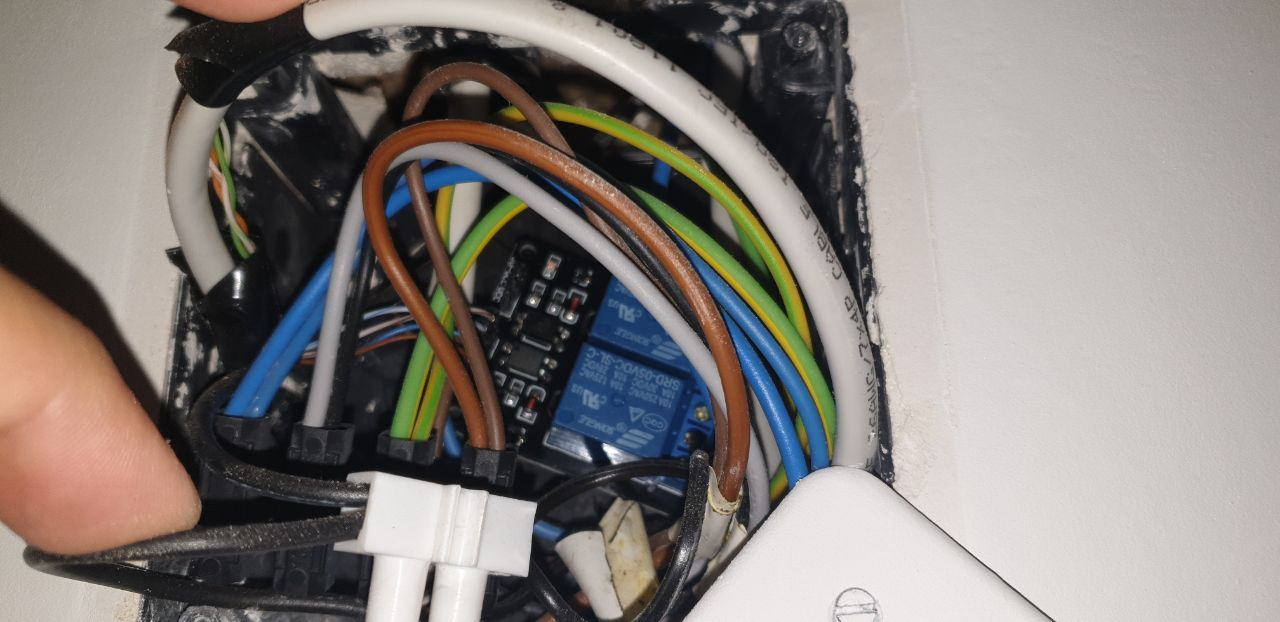
\includegraphics[width=0.9\textwidth]{img/fotos/caja-persiana.jpeg}
    \caption{Caja de derivación secundaria instalada.} \label{Img:CajaDerivacion}
\end{figure}
\begin{figure}
    \centering
    \includegraphics[width=0.9\textwidth]{img/fotos/explicación caja instalada.jpg}
    \caption{Caja de derivación principal instalada.} \label{Img:CajaDerivacionPrincipal}
\end{figure}
\begin{figure}
    \centering
    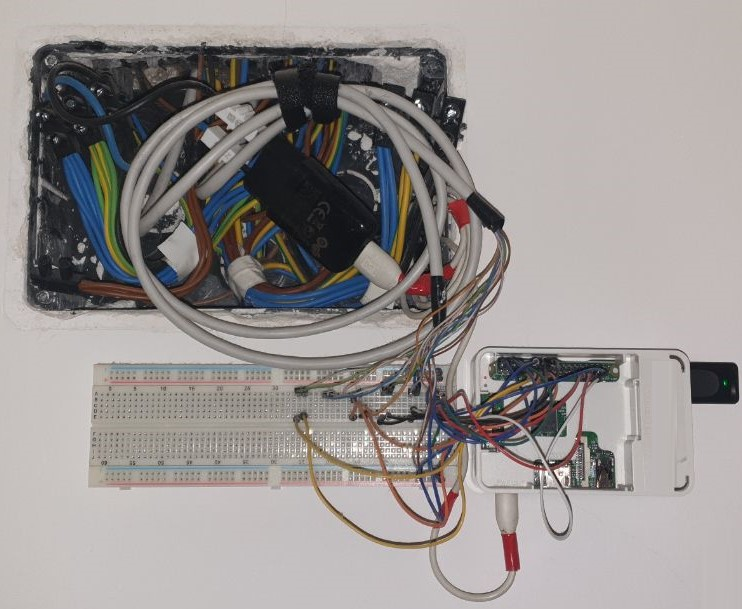
\includegraphics[width=0.9\textwidth]{img/fotos/RBP-instalada.jpeg}
    \caption{Instalación domótica y caja de derivación principal.} \label{Img:InstalacionDomotica}
\end{figure}
\begin{figure}
    \centering
    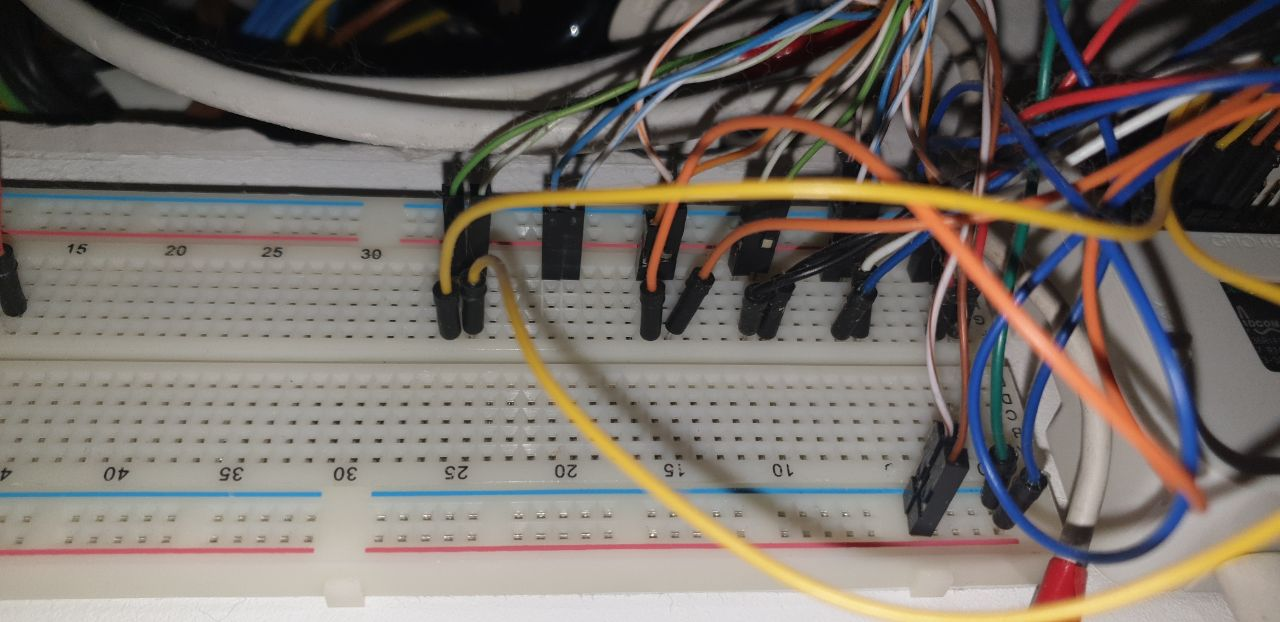
\includegraphics[width=0.9\textwidth]{img/fotos/protoboard-instalada.jpeg}
    \caption{Protoboard conectada.} \label{Img:ProtoboardConecada}
\end{figure}

Tras valorar la información y la toma de decisiones hice la instalación física quedando del siguiente modo:
\begin{itemize}
    \item En la imagen~\ref{Img:CajaDerivacion} podemos ver una caja de derivación donde ya tenemos albergada la placa de relés. 
    \item En la imagen~\ref{Img:CajaDerivacionPrincipal} vemos la caja de derivación principal con la instalación terminada indicando algunos elementos.
    \item En la imagen~\ref{Img:InstalacionDomotica} vemos la situación final de la tirada de cable y conectorizado.
    \item En la imagen~\ref{Img:ProtoboardConecada} podemos diferenciar que existen dos tipos de conectores. Los redondos ya vienen conectorizados de fábrica pero los cuadrados los he fabricado según las necesidades. Estos conectores cuadrados son del tipo~\href{https://ae01.alicdn.com/kf/H4205e9c4ec4c4be4864e44b6925a22bdf/10-juegos-de-conector-de-Cable-de-2-54mm-XH2-54-conector-XH-macho-y-hembra.jpg_Q90.jpg_.webp}{JST-XH}.
\end{itemize}

\begin{figure}
    \centering
    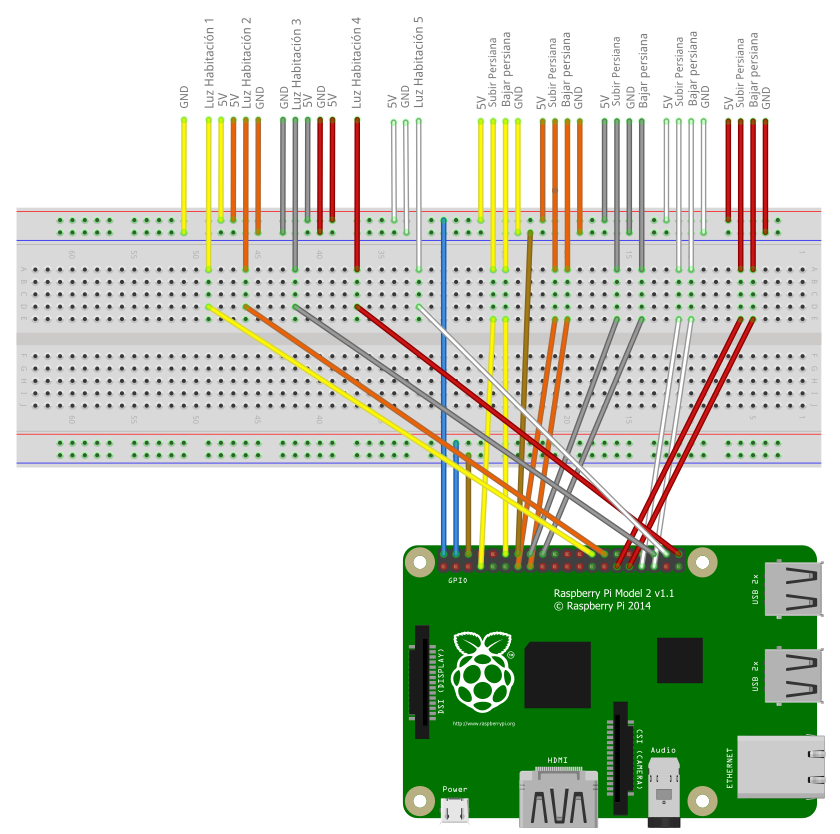
\includegraphics[width=0.9\textwidth]{img/RbP_CompletaLineas.png}
    \caption{Conectorizado final de las líneas GPIO.} \label{Img:RbP_CompletaLineas}
\end{figure}

El conectorizado final de las salidas de los GPIO es el que se puede ver en la imagen~\ref{Img:RbP_CompletaLineas}

Podemos interactuar con los puertos GPIO desde Bash y desde Python~\cite{misc:Python}. Se ha decidido utilizar lenguaje Bash para interactuar con los GPIO, dejando la potencia de Python para la obtención y procesado de datos. En ocasiones se producen errores al lanzar desde Cron scripts Python, por lo que se lanzará todo desde scripts bash.


\subsection{Diagramas eléctricos}
Para mayor claridad he generado unos planos eléctricos para aclarar como se ha realizado la instalación.

\begin{figure}
    \centering
    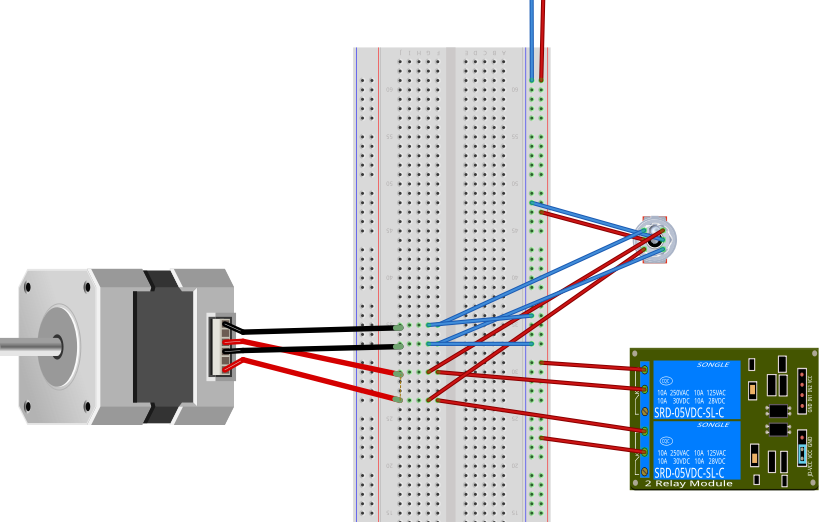
\includegraphics[width=0.9\textwidth]{img/Diagramas/rele-pulsador-motor.png}
    \caption{Raspberry Pi, relé y pulsador.} \label{Img:Relé+Pulsador+Rbp_Fritzing}
\end{figure}
\begin{figure}
    \centering
    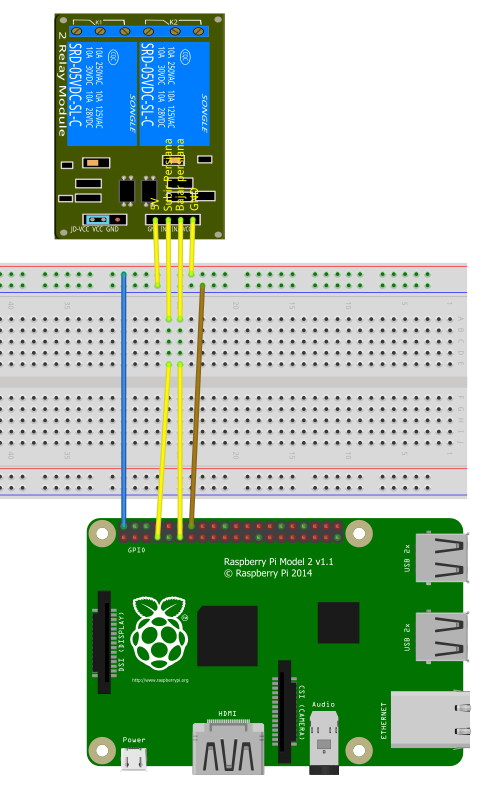
\includegraphics[width=0.5\textwidth]{img/Diagramas/relé-RBP.png}
    \caption{Raspberry y relé conectados.} \label{Img:Relé+Rbp_Fritzing}
\end{figure}

\begin{itemize}
    \item En la imagen~\ref{Img:Relé+Pulsador+Rbp_Fritzing} podemos ver que tenemos conectada una placa con dos relés y un pulsador en paralelo, con el motor de la persiana. La protoboard realmente no existe en este punto pero la he incluido para clarificar el circuito.
    \item En la imagen~\ref{Img:Relé+Rbp_Fritzing} podemos ver como se conecta el relé a una persiana identificando cada uno de los pines.
\end{itemize}

\begin{figure}
    \centering
    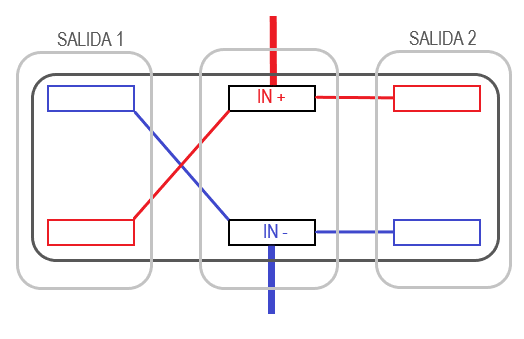
\includegraphics[width=0.6\textwidth]{img/Diagramas/PulsadorInterno.png}
    \caption{Funcionamiento interno de un pulsador para persianas.} \label{img:PulsadorInterno}
\end{figure}

Para explicar el funcionamiento de un pulsador de 3 posiciones para persianas podemos ver la imagen~\ref{img:PulsadorInterno}. En ella podemos ver como en la posición central no tiene ninguna salida, pero en la salida 1 el orden de salida de cabes es (+/-) y en la salida 2 el orden de salida de cables es (-/+). La lógica del cambio de orden en la salida de cables es porque según el sentido de la polaridad el motor girará en un sentido o en otro. Esto se respalda mediante la~\href{https://fisica.laguia2000.com/dinamica-clasica/fuerzas/ley-de-laplace-fuerza-ejercida-sobre-un-conductor}{segunda ley de Laplace} para cada espira del bobinado del motor quedando de la forma~\href{http://www.uco.es/grupos/giie/cirweb/teoria/tema_11/tema_11_01.pdf}{$M=N*(I*B*l+sen\theta)$}.

Siguiendo esta lógica, podemos ver que en la imagen~\ref{Img:Relé+Pulsador+Rbp_Fritzing} tenemos dos relés de forma que cada uno de ellos deja pasar la corriente en un sentido. En la realidad, el motor no tiene por qué tener dos entradas positivas y dos negativas pero en el dibujo queda mejor ilustrado que son entradas diferentes.

Resumiendo, la instalación mecánica y nuestra instalación mediante relés se instalarán en paralelo para poder activar una opción o la otra según la ocasión.

\subsection{Pruebas Físicas}

\begin{figure}
    \centering
    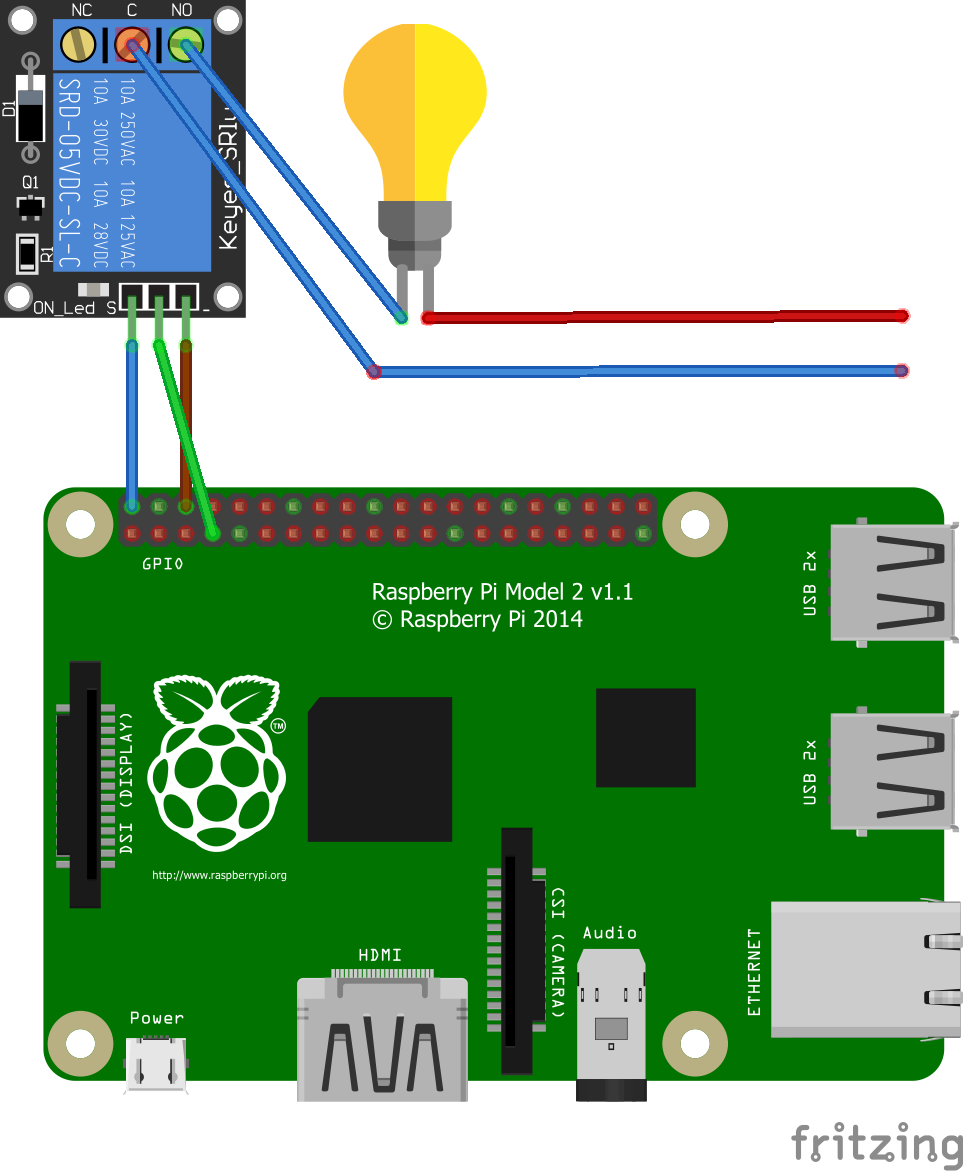
\includegraphics[width=0.6\textwidth]{img/Plano_Placa_Pruebas.png}
    \caption{Plano de tablero de pruebas.} \label{Img:Plano_Placa_Pruebas}
\end{figure}

La primera prueba, consistía en la instalación de la Raspberry Pi (Ver imagen~\ref{Img:Especificaciones RBP2B}), con un relé (ver imagen~\ref{Img:Rele1}) y una bombilla conectada a 220VAC\footnote{VAC:Voltage Alternating Current}, y se llevó a cabo con éxito. Podemos ver un diagrama de como se conectó en la imagen~\ref{Img:Plano_Placa_Pruebas}.

Llegados a este punto, era interesante el comprobar que se podía lanzar correctamente un script de este tipo desde CRON, encendiendo y apagando la bombilla, que también fue un éxito.

La tirada de cable y conectorizado en todo el domicilio, desde la primera caja de empalmes a las 5 persianas ya que es el punto del domicilio donde se recogen los cables eléctricos que llegan hasta las persianas, quedó como podemos ver en el diagrama~\ref{Img:diagramaBasico}. 

\subsection{Automatizado y puesta a producción}
Una vez se tienen las funcionalidades de los scripts corriendo correctamente, debemos asegurar las funciones y métodos de nuestra aplicación ante posibles fallos utilizando try/except. De esta manera siempre sabremos si se han actualizado correctamente los datos necesarios para que modifique nuestro Cron reportando un mensaje de error en caso contrario.

Para poder generar el proceso de que hablamos en la imagen~\ref{Img:Cron1} no es necesario salvar la cabecera del archivo de configuración de Cron, pero en nuestro caso, haremos una copia de la cabecera de forma que nuestra manipulación sea lo menos intrusiva posible. De esta manera, generaremos un Cron similar al que tenemos <<de serie>> pero con nuestras líneas de lanzado de scripts.
En ese punto he tenido problemas al intentar ejecutar scripts Python desde Cron impidiendo que se obtuvieran los datos.

Uno de los puntos de la automatización es la generación de un demonio para nuestro bot de forma que se ejecutará con el inicio del sistema y podremos trabajar con el una sencilla sentencia:

\begin{lstlisting}[language=cpp,firstnumber=0]
sudo systemctl bot stop
\end{lstlisting}
\begin{lstlisting}[language=cpp]
sudo systemctl bot start 
\end{lstlisting}
Para conseguirlo, he realizado los siguientes pasos:

He generado el archivo el archivo de nuestro demonio en lib/systemd/system/ con la extensión <<.service>>. Lo he escrito fácilmente con nano: 
\begin{lstlisting}[language=cpp, firstnumber=0]
sudo nano /lib/systemd/system/bot.service
\end{lstlisting}
El contenido del archivo es:
\begin{lstlisting}[language=cpp, caption={Modificaciones en el archivo /lib/systemd/system/bot.service.}, firstnumber=0]
[Unit]
Description=Lanza el bot de control domótico
After=network.target
StartLimitIntervalSec=0

[Service]
Type=simple
Restart=always
RestartSec=1
User=pi
WorkingDirectory=/home/pi/source/TFG/scripts/bot/
ExecStart=/usr/bin/env python3 /home/pi/source/TFG/scripts/bot/bot.py

[Install]
WantedBy=multi-user.target
\end{lstlisting}
Después debemos actualizar los demonios con: 
\begin{lstlisting}[language=cpp, firstnumber=0]
systemctl daemon-reload
\end{lstlisting}
Iniciar el demonio: 
\begin{lstlisting}[language=cpp, firstnumber=0]
sudo systemctl start bot
\end{lstlisting}
Parar el demonio: 
\begin{lstlisting}[language=cpp, firstnumber=0]
sudo systemctl stop bot
\end{lstlisting}
Estado del demonio, con el que podremos conocer el pid~\footnote{Identificador del proceso}, que siempre es útil: 
\begin{lstlisting}[language=cpp, firstnumber=0]
sudo systemctl status bot
\end{lstlisting}

Para incluirlo en el inicio de la máquina habría que moverlo a /etc/init.d y luego ejecutar: 
\begin{lstlisting}[language=cpp, firstnumber=0]    
sudo update-rc.d bot defaults
sudo systemctl daemon-reload
sudo systemctl enable bot
sudo systemctl start bot
\end{lstlisting}  


\subsection{Telegram Bot}\label{5.TelegramBot}
En primer lugar, explicaré que es un bot

El medio de comunicación con el sistema domótico es un bot de Telegram que he diseñado y programado para hacer completamente funcional el proyecto. Desde el Bot, podemos controlar las persianas de forma instantánea, modificar la configuración del sistema domótico y simulador de presencia, volver a generar recolección de datos y el grabado de los archivos. También podemos obtener información sobre la información recopilada, sobre nuestra Raspberry Pi y sobre el funcionamiento futuro del sistema domótico y simulador de presencia.

Afortunadamente estaba mejor documentado que el resto del proyecto pero aún así no ha resultado tarea fácil entender la lógica del bot. 
Podemos ver la lógica de comunicaciones del bot en la imagen~\ref{Img:FuncionamientoBot}. 

\begin{figure}
    \centering
    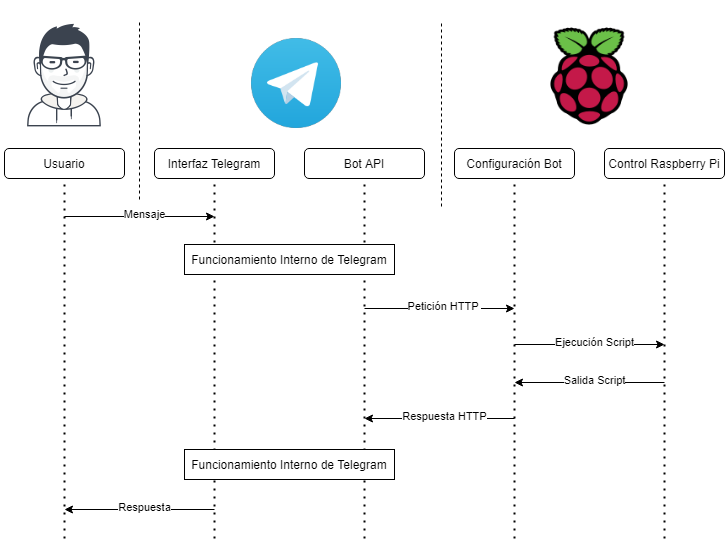
\includegraphics[width=1.0\textwidth]{img/Diagramas/FuncionamientoBot.png}
    \caption{Comunicación del bot. } \label{Img:FuncionamientoBot}
\end{figure}

Todos los mensajes de Telegram que llegan a nuestro bot, tienen la siguiente estructura json:

\begin{lstlisting}[language=json,firstnumber=0, basicstyle=\small, caption={Contenido de un mensaje de Telegram.}]
{
    'content_type':'text',
    'id':0000,
    'message_id':0000,
    'from_user':{
        'id':000000000,
        'is_bot':False,
        'first_name':'David',
        'username':'David',
        'last_name':'David',
        'language_code':'es',
        'can_join_groups':None,
        'can_read_all_group_messages':None,
        'supports_inline_queries':None
    },
    'date':1609105539,
    'chat':{
        'id':000000000,
        'type':'private',
        'title':None,
        'username':'David',
        'first_name':'David',
        'last_name':'David',
        'all_members_are_administrators':None,
        'photo':None,
        'description':None,
        'invite_link':None,
        'pinned_message':None,
        'permissions':None,
        'slow_mode_delay':None,
        'sticker_set_name':None,
        'can_set_sticker_set':None
    },
        'forward_from':None,
        'forward_from_chat':None,
        'forward_from_message_id':None,
        'forward_signature':None,
        'forward_sender_name':None,
        'forward_date':None,
        'reply_to_message':None,
        'edit_date':None,
        'media_group_id':None,
        'author_signature':None,
        'text':'a',
        'entities':None,
        'caption_entities':None,
        'audio':None,
        'document':None,
        'photo':None,
        'sticker':None,
        'video':None,
        'video_note':None,
        'voice':None,
        'caption':None,
        'contact':None,
        'location':None,
        'venue':None,
        'animation':None,
        'dice':None,
        'new_chat_member':None,
        'new_chat_members':None,
        'left_chat_member':None,
        'new_chat_title':None,
        'new_chat_photo':None,
        'delete_chat_photo':None,
        'group_chat_created':None,
        'supergroup_chat_created':None,
        'channel_chat_created':None,
        'migrate_to_chat_id':None,
        'migrate_from_chat_id':None,
        'pinned_message':None,
        'invoice':None,
        'successful_payment':None,
        'connected_website':None,
        'reply_markup':None,
        'json':{
        'message_id':0000,
        'from':{
        'id':000000000,
        'is_bot':False,
        'first_name':'David',
        'last_name':'David',
        'username':'David',
        'language_code':'es'
    },
    'chat':{
        'id':000000000,
        'first_name':'David',
        'last_name':'David',
            'username':'David',
        'type':'private'
    },
    'date':1609105539,
    'text':'a'
    }
}
\end{lstlisting}

De esta estructura utilizamos únicamente unos pocos y podríamos resumir en los siguientes:
\begin{lstlisting}[language=json,firstnumber=0, basicstyle=\small, caption={Resumen de los datos que utilizamos del mensaje de Telegram.}]
{
    'content_type':'text',
    'message_id':0000,
    'text':'a',
    'chat':{
        'id':000000000,
        'first_name':'David',
        'last_name':'David',
        'username':'David'}
}
\end{lstlisting}

Al comienzo del proyecto pensé en crear un grupo de usuarios para gestionar esta información pero he creído oportuno que cada usuario tenga su propia interfaz aunque realmente no habría problema en hacerlo de esta manera y hubiera facilitado el proyecto. Esto se ha solucionado incluyendo la lista de usuarios que pueden interactuar con el bot en el archivo de configuración. Para este paso, debemos recoger el id del usuario. Este id aparece varias veces en el json que recibimos en cada mensaje por lo que valdría cualquiera de ellos. Para el resumen he escogido el id que pertenece al objeto chat, junto al nombre y apellidos del propietario y el nombre de usuario.
El número de usuario es necesario para saber a quién le enviamos el mensaje. Por ejemplo, al comienzo del bot del proyecto tenemos las siguientes líneas:

\begin{lstlisting}[language=Python]
for usuario in usuarios:
    bot.send_message(usuario, "Iniciando Sistema a las "+str(hora))
\end{lstlisting}

Estas líneas envían un mensaje de inicio con la hora a la que se produce el evento a cada uno de los usuarios de la lista de admitidos.

Otro de los puntos necesarios es el de texto que envía el usuario. Gracias a éste obtendremos la orden que enviamos por Telegram y podremos actuar en consecuencia.
Hay un punto a tener en cuenta para comprender el funcionamiento del bot, éste radica en las líneas que hay al principio de cada uno de los métodos de que dispone el bot:

\begin{lstlisting}[language=Python]
@bot.message_handler(commands=['temp'])
@bot.message_handler(func=lambda message: message.text == "t")
@bot.message_handler(func=lambda message: message.text == "T")
def command_long_text(m):
    usuario = m.chat.id
    if (compruebaUsuario(m)):
        temperaturasManana.temperaturas(m , bot)
\end{lstlisting}

En ellas podemos ver, por orden, el comando temp, al que podemos acceder enviando el comando /temp. Posteriormente vemos dos funciones lambda, éstas significan que si introducimos únicamente esa letra también lanzará el método. He introducido estos comandos rápidos para facilitar la introducción de órdenes.
Observamos que si el usuario que escribe está en la lista de admitidos, lanzará el método temperaturas pasándole el mensaje enviado y el objeto bot, que contiene información sobre el usuario y el mensaje que envía.
Por último, el método al que se llama, recoge esta información y opera en consecuencia según lo que se le pida, bien con una función u otro método.